\chapter{Gas Processes}
\label{chapter:gas_processes}

This chapter will be distributed separately, some time in October or
November.

% \section{Introduction}

% \newpage

%\section*{Problems}
%\markright{PROBLEMS}

%\begin{problem} 
% Three identical gas-cylinder systems are compressed from the
% same initial state to final states that have the same volume, one
% isothermally, one adiabatically, and one isobarically. Which
% system has the most work done on it? The least?
%\label{prob:}
%\end{problem}

%\begin{problem}
% By what factor must the volume of a gas with $\gamma = 1.4$ be
% changed in an adiabatic process if the kelvin temperature is to
% double?
%\label{prob:}
%\end{problem}

%\begin{problem}
% By how much does the temperature of (a) an ideal monatomic
% gas and (b) an ideal diatomic gas (with molecular rotation but no
% vibration) change in an adiabatic process in which $2.5\units{kJ}$ 
% of work id done on each mole of gas?
%\label{prob:}
%\end{problem}

%\begin{problem}
%An ideal gas expands to 10 times its original volume, main-
%taining a constant $440\units{K}$ temperature. If the gas does 
%$3.3\units{kJ}$ of work on its surroundings, (a) how much heat 
%does it absorb, and (b) how many moles of gas are there?
%\label{prob:}
%\end{problem}

%\begin{problem}
% A gas sample undergoes the cyclic process {\bf ABCA} shown in
% Fig. where {\bf AB} is an isotherm. The pressure at {\bf A} is 
% $60\units{kPa}$.  Find 
% \begin{enumerate}
% \item the pressure at {\bf B}, and 
% \item the net work done on the gas.
% \end{enumerate}
%\end{problem}


%\begin{problem}
%A $3.50\units{mol}$ sample of ideal gas with molar specific heat 
%$C = 5R/2$ is initially at a temperature $255\units{K}$  and 
%pressure $101\units{kPa}$. Determine the final
%temperature and the work done by the gas when $1.75\units{kJ}$ of heat
%are added to the gas 
%\begin{enumerate}
%\item isothermally, 
%\item at constant volume, and
%\item isobarically.
%\end{enumerate}
%\end{problem}

%\begin{problem}
%The curved path in Fig. lies on the $350\units{K}$ isotherm for an
%ideal gas with $\gamma = 1.4$
%\begin{enumerate}
%\item Calculate the net work done on the
%gas as it goes around the cyclic path {\bf ABCA}. 
%\item How much heat flows into or out of the gas on the 
%segment {\bf AB}?
%\end{enumerate}
%\label{prob:}
%\end{problem}

%\begin{problem}
%The curved path in Fig. lies on the $350\units{K}$ isotherm for an
%ideal gas with $\gamma = 1.4$
%\begin{enumerate}
%\item Calculate the net work done on the
%gas as it goes around the cyclic path {\bf ACDA}. 
%\item How much heat flows into or out of the gas on the 
%segment {\bf CD}?
%\end{enumerate}
%\label{prob:}
%\end{problem}



%\begin{problem}
%A $0.25\units{mol}$ sample of ideal gas initially occupies 
%$3.5\units{L}$. If it takes $61\units{J}$ of work to 
%compress the gas isothermally to $3.0\units{L}$, what's
%the temperature of the gas?
%\label{prob:}
%\end{problem}

%\begin{problem}
%A ideal gas sample undergoes the cyclic process {\bf ABCA} shown in
%Fig. , where {\bf AB} is an isotherm. The pressure at {\bf A} is 
%$60\units{kPa}$.
%Find 
%\begin{enumerate}
%\item the pressure at {\bf B}, and 
%\item the net work done on the gas.
%\end{enumerate}
%   \begin{figure}[h]
%   \begin{center}
%   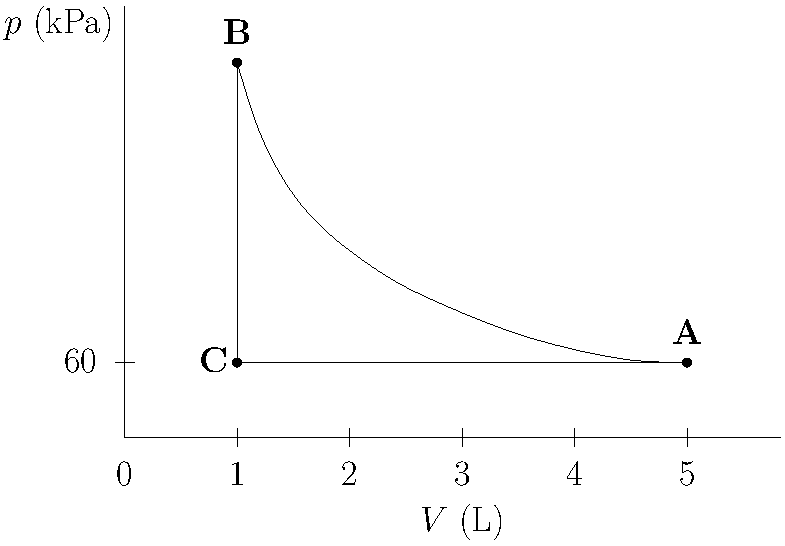
\includegraphics[width=3.0in]{gas_processes/cycle_w_isotherm_prob.pdf} 
%  \end{center} 
%   \caption{$p$-$V$ diagram for Problem \ref{prob:cycle_w_isotherm}}
%   \end{figure}
%\label{prob:cycle_w_isotherm}
%\end{problem}

%\begin{problem}
%An ideal gas with $\gamma = 1.4$ and $T = 300\units{K}$ starts at 
%point {\bf A} in Fig. It is   
%compressed adiabatically until its volume is $2.0\units{L}$ at {\bf B},
%and it is then cooled at constant pressure until it reaches $300\units{K}$
%at {\bf C}.  Finally it is allowed to expand isothermally back to 
%state {\bf A}.  Find 
%\begin{enumerate}
%\item the net work done on the gas, and 
%\item the minimum volume of the gas.
%\end{enumerate}
%\label{prob:}
%\end{problem}
%\newpage

%\begin{problem}
%A gas sample with the specific heat ratio $\gamma = 1.4$ undergoes 
%the cyclic process {\bf ABCA} shown in Fig. , where {\bf AB} is an adiabat. 
%The pressure at {\bf A} is $60\units{kPa}$.  Find 
%\begin{enumerate}
%\item the pressure at {\bf B}, and 
%\item the net work done on the gas.
%\end{enumerate}
%\begin{figure}[h]
%   \begin{center}
%   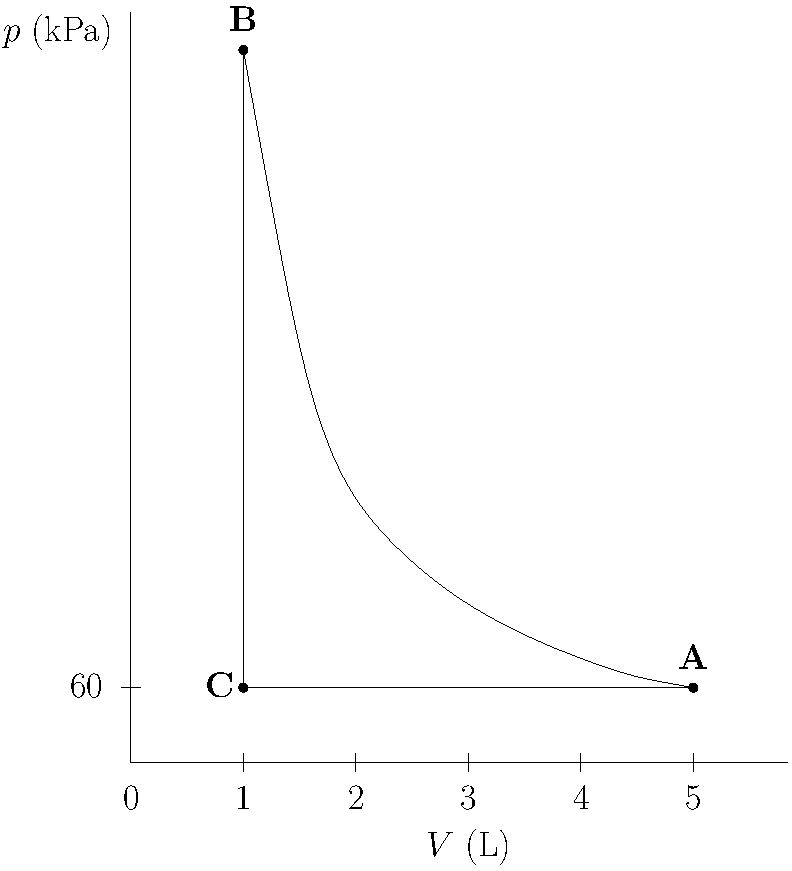
\includegraphics[width=2.5in]{gas_processes/cycle_w_adiabat_prob.pdf} 
%   \end{center} 
%   \caption{$p$-$V$ diagram for Problem \ref{prob:cycle_w_adiabat}}
%   \end{figure}
%\label{prob:cycle_w_adiabat}
%\end{problem}



